%% ECLAIR — Constraints (Springer) submission
%% Special Issue: Large Language Models for Combinatorial Constraint
%% Solving (track "SI: Large Language Models for Combinatorial
%% Constraint Solving"; deadline 2026-10-01 — see CFP.md)
%% Build: pdflatex main && bibtex main && pdflatex main && pdflatex main

\documentclass[pdflatex,sn-mathphys-num]{sn-jnl}

\usepackage{amsmath,amssymb,amsthm}
\usepackage{booktabs}
\usepackage{graphicx}
\usepackage{algorithm}
\usepackage{algpseudocode}
\usepackage{tikz}
\usetikzlibrary{arrows.meta,positioning,fit}

\theoremstyle{thmstyleone}
\newtheorem{theorem}{Theorem}
\newtheorem{proposition}[theorem]{Proposition}
\newtheorem{corollary}[theorem]{Corollary}
\newtheorem{lemma}[theorem]{Lemma}
\theoremstyle{thmstyletwo}
\newtheorem{assumption}{Assumption}
\newtheorem{remark}{Remark}
\newtheorem{definition}{Definition}

\newcommand{\Eproc}{E}
\newcommand{\Filt}{\mathcal{F}}
\newcommand{\HO}{H_0}

\raggedbottom

\begin{document}

\title[Anytime-Valid Certification of LLM-Generated Constraint Models]{ECLAIR:
Anytime-Valid Certification of LLM-Generated Constraint Models with
Budget-Aware Probe Routing}

%% TODO(authors): confirm final author list and order before submission.
\author*[1]{\fnm{Quang-Vinh} \sur{Dang}}\email{vinh.dq4@buv.edu.vn}

\affil*[1]{\orgname{British University Vietnam},
\orgaddress{\city{Hung Yen}, \country{Vietnam}}}

\abstract{Large language models translate natural-language problem
descriptions into formal constraint models, but they lack the
mathematical guarantees required for formal correctness, and no ground
truth exists against which a generated model can be checked --- the
oracle problem. Existing verification approaches are heuristic
detectors: they report empirical detection rates but provide no
statistical guarantee on the model one ultimately accepts, no
principled stopping rule, and no way to decide which test to run next
under a compute budget. We introduce ECLAIR, a sequential,
anytime-valid, budget-aware certification layer. Each candidate model
carries an e-process --- a nonnegative supermartingale wealth process
--- betting against the hypothesis that the candidate is faithful,
fed by three tiers of imperfect probes: exhaustively enumerated
micro-instances, provably valid metamorphic relations, and cross-model
majority checks. Conservative calibration of the probes' null alarm
rates preserves validity under the composite null, and a Kelly-style
rule routes solver time to the candidate--probe pair with the highest
expected evidence growth per second. Ville's inequality bounds the
probability of ever falsely rejecting a faithful model by $\alpha$
under optional stopping, and e-BH selection controls the false
discovery rate over the whole generate--test--repair tournament.
On a mutation testbed of five problem families with real CP-SAT
probes, the empirical false-rejection rate is zero at every nominal
level while $87$--$94\%$ of injected faults are detected; an
end-to-end experiment with two LLM families reproduces the guarantee
on real generated models.}

\keywords{constraint modelling, large language models, e-processes,
anytime-valid inference, solver-in-the-loop verification, false
discovery rate}

\maketitle

\section{Introduction}\label{sec:intro}

Constraint programming's long-standing adoption bottleneck is the
expertise barrier: translating a problem description held in natural
language into a formal model. Large language models (LLMs) now cross
that barrier routinely --- generating CPMpy, MiniZinc, or MILP models
from plain-English specifications \cite{michailidis2024icl,
shi2025constraintllm, szeider2025cpagent} --- but they do so without
any intrinsic guarantee of correctness. A generated model that
compiles and solves is not necessarily the model that was asked for:
a misread coefficient, a dropped constraint family, or a flipped
inequality produces a plausible artifact that returns confidently
wrong optima. Because the specification exists only in natural
language, there is no oracle to compare against; this is the central
verification difficulty the field currently faces.

The question a practitioner asks of any verification layer is:
\emph{what guarantee do I get on the model I finally accept?} Existing
answers are heuristic. Detection frameworks based on metamorphic
relations or mutation-style testing report empirical detection rates,
but offer no control over the probability of certifying an unfaithful
model, no principled rule for when enough testing has been done, and
no guidance on which of many possible tests --- differing wildly in
cost and power --- to run next under a finite solver budget.
Fixed-sample statistical tools do not repair this: a
generate--test--repair loop inherently peeks at accumulating evidence
and adapts, which invalidates fixed-sample p-values and
split-conformal calibration alike.

A concrete miniature fixes ideas. A dispatcher asks for ``a knapsack
model: pick items within the truck's 120\,kg limit, maximizing value;
items 3 and 7 cannot travel together.'' A language model returns
clean CPMpy code --- but read \texttt{120} as the \emph{count} bound
of a different template, wired the weight vector where values belong,
or emitted \texttt{sum(w*x) >= cap} after seeing a covering example
in its context. Each of these artifacts compiles, solves in
milliseconds, and returns a confident number. Asking a second model
and comparing helps only if their errors differ; testing on a
hand-checkable toy instance helps only if the error manifests there;
and the practitioner who keeps testing ``until it looks fine'' has
silently destroyed the error control of whatever test they were
using. What is missing is an accounting system for the accumulated
evidence --- one that survives the practitioner's own adaptivity.

This paper introduces \textbf{ECLAIR} (E-process Certification of
LLM-generated constraint models with Adaptive Instance Routing), a
certification layer built on the game-theoretic statistics of
e-processes \cite{ramdas2023game, shafer2021testing, grunwald2024safe}.
The design follows three observations.

First, \emph{optional stopping is the workflow}. E-processes are
designed for continuous monitoring: rejecting whenever the wealth
process crosses $1/\alpha$ controls the type-I error at $\alpha$
uniformly over all stopping times (Ville's inequality
\cite{ville1939etude}), so the loop may stop the moment evidence
suffices --- a direct compute saving --- and may resume testing at any
time without penalty.

Second, \emph{probes are heterogeneous, imperfect, and dependent}.
A brute-forced micro-instance is a near-perfect oracle but expensive;
a metamorphic relation is provably false-alarm-free but weak; a
cross-model agreement check is cheap, noisy, and entangled with the
candidate pool. E-values multiply across adaptively chosen, dependent
probes as long as each factor is a valid e-variable conditionally on
the past, and we show that a conservative upper confidence bound on
each probe family's null alarm rate --- rather than an unattainable
exact null distribution --- suffices for validity under the composite
null ``this candidate is faithful.''

Third, \emph{the budget question is a portfolio question}. Choosing
which (candidate, probe) pair to run next to maximize expected
log-evidence growth per solver-second is Kelly-optimal evidence
acquisition \cite{kelly1956new, grunwald2024safe}; because the routing
decision is measurable with respect to the past, it affects power
only, never validity.

\paragraph{Contributions.}
(i)~A formal certification protocol for LLM-generated constraint
models: per-candidate e-processes over a three-tier probe pool, with
hard certificates (probes whose false-alarm probability is exactly
zero by proof) embedded as infinite e-values
(Section~\ref{sec:framework}).
(ii)~Validity theory for the composite null: conservative calibration
preserves the supermartingale property (Lemma~\ref{lem:conservative}),
yielding anytime-valid false-rejection control under arbitrary
predictable routing (Theorem~\ref{thm:validity}), false discovery rate
control over the full generate--test--repair tournament via e-BH
\cite{wang2022false} (Proposition~\ref{prop:ebh}), and a budget bound
on the expected solver time to reject an unfaithful candidate
(Proposition~\ref{prop:budget}).
(iii)~A verified probe library for five problem families ---
knapsack with conflicts, set cover, graph colouring, generalized
assignment, and on-time job selection --- including per-family
metamorphic relations proved valid at specification level
(Proposition~\ref{prop:mr}).
(iv)~An open implementation on CPMpy~\cite{guns2019cpmpy} and OR-Tools
CP-SAT~\cite{ortools} and a five-part empirical study
(Section~\ref{sec:experiments}): a mutation testbed in which validity
holds exactly at every nominal level while $87$--$94\%$ of injected
faults are caught; ablations quantifying the contribution of each
probe tier, including an empirical demonstration that pool-entangled
probes consume the conservative validity margin; a matched-budget
comparison in which the practitioner's alternatives either cannot
reject at all (single-shot, self-consistency voting) or break their
nominal level (a fixed-sample test at $0.061$, its uncorrected
peeking variant at $0.075$) while ECLAIR detects $0.905$ at exactly
zero false rejections; an end-to-end experiment with two LLM
families in which every crash-free generated model is certified
without a single false rejection; and an ambiguity study whose
honest negative result --- current models normalize boundary-language
ambiguity to the conventional reading --- sharpens where the
silent-error regime actually lives.

\section{Related work}\label{sec:related}

\paragraph{LLMs for constraint modelling.}
In-context learning pipelines translate natural-language descriptions
into CPMpy models with retrieval and self-refinement
\cite{michailidis2024icl}; benchmark suites evaluate such systems on
CSPLib-derived corpora \cite{michailidis2025cpbench}. Agentic systems
iterate modelling with solver feedback: CP-Agent
\cite{szeider2025cpagent} maintains a persistent Python session around
CPMpy, and MCP-Solver \cite{szeider2025mcp} exposes constraint solvers
to LLMs through a model context protocol. ConstraintLLM
\cite{shi2025constraintllm} targets industrial-level CP with a
neuro-symbolic architecture. All these systems \emph{generate};
ECLAIR is complementary --- it decides, with a guarantee, whether to
\emph{trust} what was generated, and can wrap any of them.

\paragraph{Testing lineage.}
Two software-testing traditions supply ECLAIR's probe vocabulary.
Metamorphic testing \cite{chen2018metamorphic} addresses the oracle
problem by checking necessary relations between outputs on related
inputs --- exactly our tier B, with the strengthening that relations
proved against the \emph{specification} of an optimization problem
have null alarm probability zero, turning a testing heuristic into a
hard certificate inside a statistical process. Mutation testing
\cite{demillo1978hints, jia2011mutation} contributes the evaluation
methodology: systematically injected faults with screened
non-equivalence are the standard way to measure a test suite's power
when real faults are scarce, and our functional-corruption testbed
(Section~\ref{sec:experiments}) is its adaptation to model
faithfulness --- with the twist that here the ``test suite'' carries
a statistical guarantee, so the mutation score is a \emph{power}
estimate under a controlled \emph{level}, not a standalone adequacy
number.

\paragraph{Verifying generated models.}
Two recent lines attack verification directly: falsification
frameworks deriving provably valid metamorphic relations from duality
and monotonicity theory, in which a violated relation certifies
unfaithfulness, and agent-based frameworks that compose test cases and
apply optimization-oriented mutation testing.%
\footnote{%
%% TODO(citations): the two verification-framework papers from the
%% CFP-period literature scan are pending verification against live
%% records (see VERIFY_CITATIONS.md) and must be cited here before
%% submission.
Full citations pending verification.} ECLAIR subsumes the binary
verdicts of such detectors as the special case of an infinite
e-value, and adds what they lack: a guarantee on the accepted model,
a stopping rule, FDR control across repairs, and budget-aware test
selection.

\paragraph{Anytime-valid inference.}
E-values and e-processes provide measures of evidence valid at
arbitrary stopping times \cite{ramdas2023game, shafer2021testing,
vovk2021evalues}; safe tests and the GROW criterion connect optimal
evidence growth to log-optimal (Kelly) betting \cite{grunwald2024safe,
kelly1956new}; betting-based confidence sequences supply the adaptive
wagering machinery \cite{waudbysmith2024estimating}; and the e-BH
procedure controls FDR under arbitrary dependence \cite{wang2022false}.
ECLAIR ports this toolkit into constraint-model verification, where,
to our knowledge, sequential anytime-valid certification has not been
attempted.

\paragraph{Why not fixed-sample or conformal tools.}
It is worth being precise about why the natural statistical
alternatives do not fit this workflow, since the certification
problem looks superficially like ordinary hypothesis testing or
distribution-free calibration. A fixed-sample test requires the
number and identity of probes to be fixed before any outcome is seen;
a generate--test--repair loop violates this at every step --- it
looks at the running evidence to decide whether to continue testing,
which probe to run next, whether to repair, and when to stop, and
each of those choices invalidates a fixed-sample p-value in the
familiar optional-stopping way. Split-conformal calibration instead
requires exchangeability between the calibration data and the test
stream; here the ``test stream'' is adaptively generated (repaired
candidates are chosen \emph{because} of earlier outcomes; probe
instances are routed by an adaptive policy), so exchangeability fails
by construction. E-processes are designed for exactly this
regime: validity is preserved under any data-dependent stopping,
continuation, and selection rule, because the guarantee is a
supermartingale property rather than a sampling-distribution
property \cite{ramdas2023game}. The practical consequence is the one
that matters operationally: the certifier may spend its budget
\emph{where the evidence points}, stop the moment a decision is
supported, and still quote the same $\alpha$.

\section{The certification problem}\label{sec:problem}

A specification $s$ is a natural-language description of a
parameterized combinatorial optimization problem, together with an
instance distribution $\mathcal{D}$ over parameter values. A
\emph{candidate} $m$ is an executable function mapping an instance
$I \sim \mathcal{D}$ to a formal model $m(I)$ whose exact optimum we
write $v_m(I) \in \mathbb{Z} \cup \{\mathrm{INFEAS}\}$. The (unknown)
faithful value $v^\ast(I)$ is the optimum of the problem $s$ actually
describes. Candidate $m$ is \emph{faithful} if
$v_m(I) = v^\ast(I)$ for $\mathcal{D}$-almost-every $I$.

Given candidates $m_1, \dots, m_k$ produced by an LLM ensemble, a
compute budget $B$ (solver-seconds), and a risk level $\alpha$, the
certifier must decide which candidates to reject, which (if any) to
certify, or whether to abstain --- without access to $v^\ast$. The
null hypothesis attached to each candidate is
\[
\HO(m):\quad m \text{ is faithful.}
\]
$\HO(m)$ is \emph{composite}: faithfulness does not determine the law
of any probe outcome, which also depends on the instance generator,
on checker noise, and (for cross-model probes) on the composition of
the surviving pool. All guarantees below therefore hold uniformly
over the null class, which we make precise through conditional
bounds on probe alarm rates.

\section{The ECLAIR framework}\label{sec:framework}

Figure~\ref{fig:arch} shows the architecture. An LLM ensemble
proposes candidates; a cheap intake gate discards code that cannot
build and solve a toy instance; every surviving candidate carries its
own e-process; a router spends the solver budget one probe at a time;
and three exits are possible --- rejection (with a counterexample
that can seed a repaired candidate), certification of a survivor by
e-BH selection, or abstention with the full evidence ledger. The
subsections follow the data flow.

\begin{figure}[t]
\centering
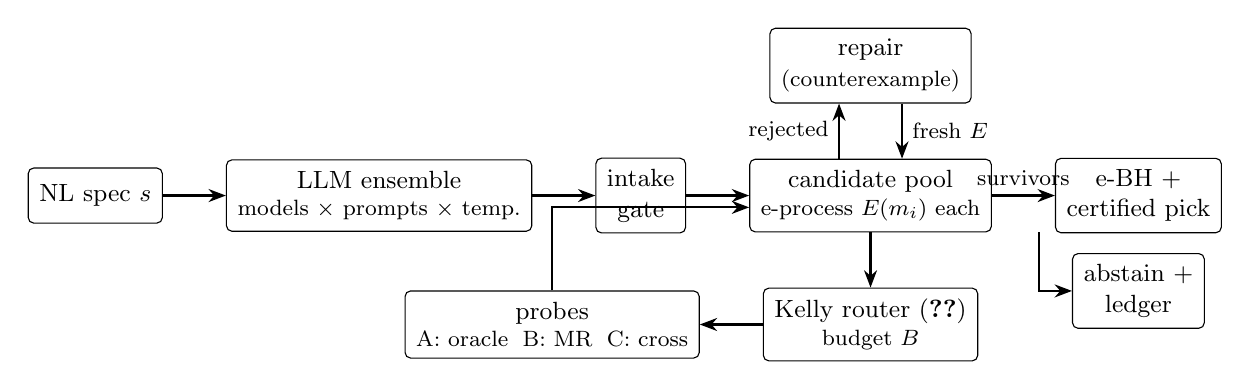
\begin{tikzpicture}[
  font=\small,
  box/.style={draw, rounded corners=2pt, align=center,
              inner sep=4pt, minimum height=7mm},
  lab/.style={font=\footnotesize, align=center},
  arr/.style={-{Stealth[length=2.2mm]}, thick}]
\node[box] (spec) {NL spec $s$};
\node[box, right=8mm of spec] (gen)
  {LLM ensemble\\[-1pt]{\footnotesize models $\times$ prompts $\times$ temp.}};
\node[box, right=8mm of gen] (gate) {intake\\gate};
\node[box, right=8mm of gate] (pool)
  {candidate pool\\[-1pt]{\footnotesize e-process $\Eproc(m_i)$ each}};
\node[box, below=7mm of pool] (router)
  {Kelly router \eqref{eq:kelly}\\[-1pt]{\footnotesize budget $B$}};
\node[box, left=8mm of router] (probes)
  {probes\\[-1pt]{\footnotesize A: oracle\; B: MR\; C: cross}};
\node[box, right=8mm of pool] (ebh)
  {e-BH +\\certified pick};
\node[box, below=2.5mm of ebh] (abstain) {abstain +\\ledger};
\node[box, above=7mm of pool] (repair) {repair\\{\footnotesize (counterexample)}};
\draw[arr] (spec) -- (gen);
\draw[arr] (gen) -- (gate);
\draw[arr] (gate) -- (pool);
\draw[arr] (pool) -- (router);
\draw[arr] (router) -- (probes);
\draw[arr] (probes) |- ([yshift=-1.5mm]pool.west);
\draw[arr] (pool) -- node[lab, above]{survivors} (ebh);
\draw[arr] ([xshift=6mm]pool.south east) |- (abstain.west);
\draw[arr] ([xshift=-4mm]pool.north) -- node[lab, left]{rejected} ([xshift=-4mm]repair.south);
\draw[arr] ([xshift=4mm]repair.south) -- node[lab, right]{fresh $\Eproc$} ([xshift=4mm]pool.north);
\end{tikzpicture}
\caption{ECLAIR's architecture. Every candidate carries its own
wealth process; the router spends the shared budget one probe at a
time; rejection feeds repair; terminal e-values enter e-BH; if
nothing survives, the evidence ledger explains why}
\label{fig:arch}
\end{figure}

\subsection{Probe tiers}\label{sec:probes}

A \emph{probe} is a randomized procedure that consumes solver time
and returns a binary alarm $X \in \{0,1\}$ against a designated
candidate. ECLAIR uses three tiers.

\paragraph{Tier A: micro-instance oracles.}
Draw an instance small enough for exhaustive enumeration of the
specification's decision space using an executable feasibility
checker, and alarm iff the candidate's exact optimum differs from the
enumerated optimum. With an exact checker the null alarm probability
is zero; in general the checker itself is imperfect (in a fully
LLM-generated pipeline it is LLM-compiled and validated by
cross-agreement), so tier A is treated as a calibrated noisy probe.

\paragraph{Tier B: metamorphic relations (hard certificates).}
A metamorphic relation (MR) transforms an instance $I$ into $I'$ such
that the specification provably implies a relation between $v^\ast(I)$
and $v^\ast(I')$ --- e.g.\ enlarging a knapsack capacity cannot
decrease the optimum, deleting a graph edge cannot increase the
chromatic number, consistently permuting item data leaves the optimum
unchanged. The probe solves the \emph{candidate} on both sides
exactly and alarms iff the relation is violated. For a faithful
candidate the alarm probability is exactly zero: both solves return
true optima of instances of the true specification, and the relation
holds for the specification by proof. A tier-B alarm is therefore a
\emph{hard certificate} of unfaithfulness.

\paragraph{Tier C: cross-model majority checks.}
Solve the designated candidate and up to three surviving partners on
a fresh mid-size instance (beyond enumeration reach --- this tier's
purpose); alarm iff at least two partners agree on a value and the
candidate deviates from that majority. Tier C is cheap and noisy, and
its null alarm rate depends on the pool: a faithful candidate alarms
when a wrong majority forms. This entanglement is handled by
calibration (Section~\ref{sec:calibration}) and is quantified
empirically in Section~\ref{sec:ablation}.

\subsection{Betting and conservative calibration}\label{sec:calibration}

Let $\Filt_{t-1}$ denote everything observed before the $t$-th probe.
For a tier-B probe the e-factor is $e_t = 1$ on pass and
$e_t = \infty$ on alarm. For tiers A and C, ECLAIR bets a Bernoulli
likelihood ratio
\begin{equation}\label{eq:bet}
e_t \;=\;
\Bigl(\tfrac{p_1}{\bar p_0}\Bigr)^{X_t}
\Bigl(\tfrac{1-p_1}{1-\bar p_0}\Bigr)^{1-X_t},
\end{equation}
where $\bar p_0$ is a \emph{conservative} (upper confidence) bound on
the tier's null alarm rate and $p_1 \in (\bar p_0, 1)$ a working
detection rate; both come from a held-out calibration corpus of
known-faithful models and screened mutants, with $\bar p_0$ the
Clopper--Pearson upper bound \cite{clopper1934use} at confidence
$97.5\%$. Only $\bar p_0$ matters for validity; $p_1$ tunes power.

\begin{lemma}[Conservative bets are safe]\label{lem:conservative}
Let $X \in \{0,1\}$ satisfy
$\Pr(X = 1 \mid \Filt_{t-1}) \le \bar p_0$ almost surely under
$\HO$, and let $e$ be given by \eqref{eq:bet} with
$0 < \bar p_0 < p_1 < 1$. Then
$\mathbb{E}[\,e \mid \Filt_{t-1}\,] \le 1$ under $\HO$.
\end{lemma}

\begin{proof}
With $q = \Pr(X{=}1 \mid \Filt_{t-1})$,
$\mathbb{E}[e \mid \Filt_{t-1}]
= q\,\frac{p_1}{\bar p_0} + (1-q)\,\frac{1-p_1}{1-\bar p_0}$,
which is affine and increasing in $q$ because
$p_1/\bar p_0 > 1 > (1-p_1)/(1-\bar p_0)$. At $q = \bar p_0$ it equals
$p_1 + (1-p_1) = 1$; hence for $q \le \bar p_0$ it is at most $1$.
\end{proof}

The candidate's wealth process is the running product
$\Eproc_t(m) = \prod_{s \le t,\, s \to m} e_s$ over the probes routed
to $m$, with $\Eproc_0(m) = 1$.

\paragraph{The betting arithmetic, numerically.}
With the calibrated values of Section~\ref{sec:experiments}
(Table~\ref{tab:calib}), the multipliers of \eqref{eq:bet} are
concrete: a tier-A alarm multiplies wealth by
$p_1/\bar p_0 = 0.473/0.0153 \approx 31$, a pass by
$(1{-}p_1)/(1{-}\bar p_0) \approx 0.53$; a tier-C alarm multiplies by
${\approx}3.0$, a pass by ${\approx}0.61$; tier B multiplies by $1$
on pass and rejects outright on alarm. Against the rejection
threshold $1/\alpha = 20$ this means: a single tier-A alarm brings a
fresh candidate to within one small step of rejection
($\log 31 > \log 20$ already, from wealth $1$); two early tier-A
passes push a candidate's wealth down to ${\approx}0.28$, after which
the Kelly numerator of \eqref{eq:kelly} for noisy tiers turns
negative and the router parks the candidate on zero-bleed tier-B
probes --- exactly the flattening visible in
Figure~\ref{fig:trajectories}. The asymmetry (alarm evidence
${\sim}31\times$, pass evidence ${\sim}0.53\times$) is not a tuning
choice but the likelihood-ratio geometry of a rare-under-null,
common-under-alternative event.

\subsection{Budget-aware routing}\label{sec:routing}

At each step ECLAIR selects
\begin{equation}\label{eq:kelly}
(m, p)^\star \;=\; \arg\max_{(m,p)}\;
\frac{\mathbb{E}\bigl[\log e \,\bigm|\, q_m\bigr]}{c(p)},
\end{equation}
the candidate--probe pair maximizing expected log-wealth growth per
solver-second: Kelly-optimal evidence acquisition in the sense of the
GROW criterion \cite{grunwald2024safe, kelly1956new}. Here $q_m$ is a
running (Bayes) posterior that $m$ is unfaithful, maintained with the
same calibrated rates and used \emph{only} for routing; $c(p)$ is the
tier's calibrated mean cost. For tiers A/C the numerator is
$q_m G_1 + (1-q_m) G_0$ with $G_1, G_0$ the expected log-factors of
\eqref{eq:bet} under alarm rates $p_1, \bar p_0$; for tier B it is
$q_m\,\delta_B \bigl(\log(1/\alpha) - \log \Eproc_t(m)\bigr)$, the
calibrated hard-certificate rate times the remaining log-gap to the
rejection threshold. Because \eqref{eq:kelly} is
$\Filt_{t-1}$-measurable, routing affects power only --- validity is
untouched (Theorem~\ref{thm:validity}).

\subsection{Decisions, repair, and abstention}\label{sec:decisions}

Candidate $m$ is \emph{rejected} the first time
$\Eproc_t(m) \ge 1/\alpha$ (or on a tier-B alarm). A rejected
candidate may be \emph{repaired}: the violating probe is fed back to
the LLM as a counterexample and the repaired candidate enters the
pool as a fresh e-process. When the budget is exhausted (or one
candidate's survival dominates), the terminal e-values of \emph{all}
candidates ever considered enter the e-BH procedure
\cite{wang2022false} at level $\alpha$; among Ville-survivors the
candidate with the smallest e-value is the certified output, together
with its evidence ledger. If no candidate survives, ECLAIR
\emph{abstains} and returns the ledger --- a structured explanation of
which probes killed every reading of the specification, which doubles
as a signal for conversational re-elicitation.
Algorithm~\ref{alg:eclair} summarizes the loop.

\begin{algorithm}[t]
\caption{ECLAIR}\label{alg:eclair}
\begin{algorithmic}[1]
\Require spec $s$, candidates $m_1{:}k$, budget $B$, level $\alpha$,
         calibrated $(\bar p_0, p_1, \delta_B, c)$ per tier
\State $\Eproc(m_i) \gets 1$, $q_{m_i} \gets q_{\mathrm{prior}}$ for all $i$
\While{$B > 0$ \textbf{and} some candidate alive}
  \State $(m, p) \gets$ maximizer of \eqref{eq:kelly} over alive
         candidates and tiers
  \State run probe $p$ on $m$; observe alarm $X$, measured cost $c$;
         $B \gets B - c$
  \If{$p$ is tier B \textbf{and} $X = 1$}
     reject $m$ \Comment{hard certificate}
  \Else
     \State $\Eproc(m) \gets \Eproc(m) \cdot e(X)$ by \eqref{eq:bet};
            update $q_m$ by Bayes
     \If{$\Eproc(m) \ge 1/\alpha$} reject $m$ \EndIf
  \EndIf
  \State optionally: repair rejected $m$ via counterexample; add as
         fresh e-process
\EndWhile
\State \Return e-BH rejection set at level $\alpha$; certified pick
       $\arg\min_{\text{survivors}} \Eproc(m)$, or abstain with the
       evidence ledger
\end{algorithmic}
\end{algorithm}

\subsection{A worked run}\label{sec:worked}

Figure~\ref{fig:trajectories} traces one certified pool --- three
faithful candidates and three screened mutants of the set-cover
family --- under Kelly routing at $\alpha = 0.05$ with a $640$\,ms
budget of measured solver time. Every mechanism of the framework is
visible in the paths. Two mutants are driven across the rejection
threshold within $60$\,ms: the router's prior makes every candidate
equally suspect at the start, tier-A alarms multiply their wealth by
$p_1/\bar p_0 \approx 31$, and two to three alarms suffice. The third
mutant survives its first probes by luck, its posterior $q_m$ drops,
and the router deprioritizes it --- until the pool thins, its
relative score rises again, and a single tier-B hard certificate
(the near-vertical jump at ${\sim}290$\,ms) removes it. The faithful
candidates' paths tell the validity story: early tier-A/C passes
drive their wealth \emph{down} (a pass multiplies by
$(1-p_1)/(1-\bar p_0) < 1$), after which the router --- seeing low
$q_m$ --- feeds them almost exclusively zero-bleed tier-B probes, so
their wealth flattens far below the threshold and the remaining
budget is spent where Lemma~\ref{lem:conservative} makes passes free.
The certified pick is the faithful candidate with the smallest
terminal wealth; its ledger records every probe shown in the figure.
Table~\ref{tab:trace} lists the first fourteen ledger entries
verbatim: the entire decision logic of the framework --- likelihood
ratios, threshold crossings, router hand-offs to the zero-bleed tier
--- is legible in fourteen rows of arithmetic.

\begin{table}[t]
\caption{The first fourteen ledger entries of the run in
Figure~\ref{fig:trajectories} ($m_1$--$m_3$ faithful, $m_4$--$m_6$
mutants; $\alpha = 0.05$, rejection at
$\log \Eproc \ge \log 20 \approx 3.00$). Steps 4--5: one tier-A alarm
each rejects $m_4, m_5$ outright ($\log 31.0 = 3.43$). The lucky
mutant $m_6$ passes its first probes and is parked, with the
faithful, on zero-bleed tier-B probes (steps 11--14) --- it is
rejected much later by a hard certificate (Fig.~\ref{fig:trajectories}).}
\label{tab:trace}
\begin{tabular}{cclcc}
\toprule
Step & Candidate & Tier & $e$-factor & $\log \Eproc$ after\\
\midrule
1--3 & $m_1, m_2, m_3$ & A (pass) & $0.535$ & $-0.626$\\
4 & $m_4$ & A (\textbf{alarm}) & $31.0$ & $3.435$ $\to$ \textbf{reject}\\
5 & $m_5$ & A (\textbf{alarm}) & $31.0$ & $3.435$ $\to$ \textbf{reject}\\
6 & $m_6$ & A (pass) & $0.535$ & $-0.626$\\
7--10 & $m_1, m_2, m_3, m_6$ & A (pass) & $0.535$ & $-1.252$\\
11--14 & $m_1, m_2, m_3, m_6$ & B (pass) & $1.000$ & $-1.252$\\
\bottomrule
\end{tabular}
\end{table}

\begin{figure}[t]
\centering
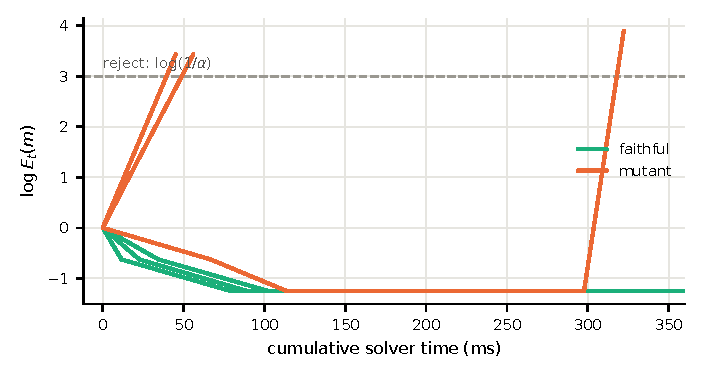
\includegraphics[width=\linewidth]{figures/Fig1}
\caption{Wealth trajectories $\log \Eproc_t(m)$ of one certified pool
(three faithful set-cover candidates, three screened mutants; Kelly
routing, $\alpha = 0.05$). Mutant paths cross the rejection threshold
(dashed); the late near-vertical jump is a tier-B hard certificate.
Faithful paths drift down on early noisy passes, then flatten as the
router shifts them to zero-bleed tier-B probes}
\label{fig:trajectories}
\end{figure}

\section{Guarantees}\label{sec:theory}

\begin{assumption}\label{ass:null}
Under $\HO(m)$: tier-B probes alarm with probability zero, and each
tier-A/C probe routed to $m$ alarms with conditional probability at
most its calibrated bound $\bar p_0$, given $\Filt_{t-1}$.
\end{assumption}

The tier-B half of Assumption~\ref{ass:null} is a theorem for the
probe library of Section~\ref{sec:experiments}
(Proposition~\ref{prop:mr}); the tier-A/C half is what conservative
calibration targets, and its empirical status --- including where it
becomes delicate --- is examined in Section~\ref{sec:ablation}.

\begin{theorem}[Anytime validity]\label{thm:validity}
Under Assumption~\ref{ass:null}, for any predictable routing rule,
any repair policy, and any stopping rule,
\[
\Pr_{\HO(m)}\bigl(\exists\, t:\ \Eproc_t(m) \ge 1/\alpha\bigr)
\;\le\; \alpha .
\]
\end{theorem}

\begin{proof}
Each factor contributed to $\Eproc(m)$ is nonnegative and, by
Lemma~\ref{lem:conservative} (tiers A/C) or by the zero-alarm
property (tier B, factor $\equiv 1$ a.s.\ under $\HO$), satisfies
$\mathbb{E}[e_t \mid \Filt_{t-1}] \le 1$; predictability of the
routing rule makes ``which probe, on which candidate'' a
$\Filt_{t-1}$-measurable choice, so the tower property gives
$\mathbb{E}[\Eproc_t(m)] \le 1$ and $\Eproc_t(m)$ is a nonnegative
supermartingale. Ville's inequality \cite{ville1939etude} concludes.
\end{proof}

\begin{proposition}[Tournament FDR control]\label{prop:ebh}
Let $\{ \Eproc(m) \}$ be the terminal e-values of all candidates
considered across all generation and repair rounds. Applying e-BH at
level $\alpha$ controls the false discovery rate of the rejected set
at $\alpha$, regardless of the dependence induced by shared probes,
common instances, pool entanglement, or data-driven repairs.
\end{proposition}

\begin{proof}
Each $\Eproc(m)$ is a valid e-value for $\HO(m)$ by
Theorem~\ref{thm:validity} (optional stopping preserves
$\mathbb{E} \le 1$). The e-BH procedure controls FDR for arbitrarily
dependent e-values \cite{wang2022false}.
\end{proof}

\begin{proposition}[Budget to rejection]\label{prop:budget}
Fix an unfaithful candidate $m$ and a routing rule under which the
probes applied to $m$ satisfy
$\mathbb{E}[\log e_t \mid \Filt_{t-1}] \ge \Delta > 0$ and
$|\log e_t| \le L$. Then the number $\tau$ of probes until rejection
satisfies
$\mathbb{E}[\tau] \le \bigl(\log(1/\alpha) + L\bigr)/\Delta$.
\end{proposition}

\begin{proof}
$M_t = \log \Eproc_t(m) - t\Delta$ is a submartingale minorant;
optional stopping for the bounded-increment stopped process at
$\tau \wedge n$ gives
$\Delta\,\mathbb{E}[\tau \wedge n] \le
\mathbb{E}[\log \Eproc_{\tau \wedge n}] \le \log(1/\alpha) + L$,
and monotone convergence lets $n \to \infty$.
\end{proof}

Proposition~\ref{prop:budget} is the quantitative content of ``stop
the moment evidence suffices'': the budget scales as
$\log(1/\alpha)$, so tightening the guarantee is cheap --- consistent
with the flat detection curves across $\alpha$ observed in
Section~\ref{sec:alpha}.

Finally, the tier-selection layer of the router admits a no-regret
guarantee. The deployed router uses the plug-in posterior form
\eqref{eq:kelly}; the following analyzes its online-learning
relative, in which the tier weights are maintained by the
exponentially weighted average (Hedge) forecaster
\cite{freund1997decision, cesabianchi2006prediction} over the
realized growth-per-cost rewards.

\begin{proposition}[No-regret tier selection]\label{prop:regret}
Fix a candidate and let $r_t(p) = \log e_t(p)/c(p) \in [-L, L]$
denote the (bounded) realized log-growth per unit cost had tier
$p \in \{A, B, C\}$ been probed at step $t$. Selecting tiers by Hedge
with learning rate $\eta = \sqrt{8 \ln 3 / T}$ guarantees
\[
\max_{p}\sum_{t=1}^{T} r_t(p) \;-\;
\mathbb{E}\Bigl[\sum_{t=1}^{T} r_t(p_t)\Bigr]
\;\le\; L\,\sqrt{(T/2)\ln 3},
\]
i.e.\ the realized evidence growth per unit cost is within
$O(\sqrt{T})$ of the best fixed tier in hindsight; since tier
selection remains $\Filt_{t-1}$-measurable, Theorem~\ref{thm:validity}
is unaffected.
\end{proposition}

\begin{proof}
Immediate from the standard Hedge regret bound for bounded rewards
over $3$ experts \cite[Thm.~2.2]{cesabianchi2006prediction}, after
rescaling $r_t$ to $[0,1]$; predictability holds because the Hedge
weights at step $t$ depend only on rewards observed before $t$.
\end{proof}

\begin{proposition}[Probe-family validity]\label{prop:mr}
For the five problem families of Section~\ref{sec:experiments}, the
implemented metamorphic relations --- capacity/deadline/cost
monotonicity, structural relaxation (conflict, edge, or coverage-row
deletion), restriction (edge addition), and consistent data
permutation --- have null alarm probability exactly zero when both
sides are solved exactly.
\end{proposition}

\begin{proof}[Proof sketch]
Each relation is proved at specification level; exact solves transfer
it to any faithful candidate. Monotone relaxations follow from
feasible-set inclusion (e.g.\ enlarging a knapsack capacity or
deleting a conflict pair only enlarges the feasible set of the
specification, so the maximum cannot decrease); objective
monotonicity follows from pointwise dominance; permutation invariance
follows from the specification's symmetry under consistent relabeling
of items, sets, vertices, or jobs. The one delicate case is deadline
extension in on-time job selection, where the constraint
\emph{indices} shift with the deadline order: there, validity follows
because the earliest-due-date feasibility conditions are equivalent
to true single-machine schedulability of the selected set, and
schedulability is monotone in deadlines. Full proofs accompany the
probe library.
\end{proof}

\begin{remark}
Assumption~\ref{ass:null} for tier C deserves emphasis: the null
alarm event ``a wrong majority forms among partners'' depends on the
surviving pool, so its conditional probability is bounded uniformly
only if calibration reflects the pool compositions actually
encountered. Section~\ref{sec:ablation} shows empirically that this
is not pedantry --- the conservative margin visibly erodes exactly,
and only, when tier C is made the sole evidence source.
\end{remark}

\section{A verified probe library for five problem families}
\label{sec:library}

The guarantees of Section~\ref{sec:theory} are only as real as
Assumption~\ref{ass:null}, and tier B's half of that assumption is a
per-relation \emph{proof obligation}. This section discharges it for
a concrete library spanning five combinatorial families chosen to
exercise packing, covering, colouring, assignment, and scheduling
structure. For each family we implement a reference model, an
independent executable checker (the tier-A enumeration oracle), and
the metamorphic relations below; full validity proofs are in
Appendix~\ref{app:proofs}. Table~\ref{tab:families} summarizes.

\begin{table}[t]
\caption{The probe library. MRs state a provable relation between the
specification optima of an instance $I$ and its transform $I'$;
$\uparrow$ ($\downarrow$) means the optimum cannot decrease
(increase), $=$ means it is unchanged. Mutation classes are the
functional corruptions used to create ground-truth unfaithful
candidates.}\label{tab:families}
\begin{tabular}{p{2.9cm}p{4.2cm}p{4.2cm}}
\toprule
Family (sense) & Metamorphic relations & Mutation classes\\
\midrule
Knapsack with conflicts (max) &
capacity$+\delta$: $\uparrow$; drop conflict: $\uparrow$; permute
items: $=$ &
capacity shift; weight/value entry; vector rotation; conflict-row
drop/half-drop; operator flip\\
\addlinespace
Set cover (min) &
drop element: $\downarrow$; cost entry$+\delta$: $\uparrow$; permute
sets: $=$ &
cost entry; coverage-row drop/half-drop; operator flip\\
\addlinespace
Graph colouring (min) &
drop edge: $\downarrow$; add edge: $\uparrow$; relabel vertices: $=$ &
edge drop/half-drop; adjacency-logic flip\\
\addlinespace
Generalized assignment (min) &
capacity$+\delta$: $\downarrow$; cost entry$+\delta$: $\uparrow$;
permute tasks: $=$ &
size/capacity entry; vector rotation; cost-matrix entry; operator
flip\\
\addlinespace
On-time job selection (max) &
deadline$+\delta$: $\uparrow$; weight$+\delta$: $\uparrow$;
processing$-\delta$: $\uparrow$; permute jobs: $=$ &
processing/deadline/weight entry; vector rotation; operator flip\\
\bottomrule
\end{tabular}
\end{table}

\paragraph{Three structural remarks.}
First, the relations fall into three provable classes ---
\emph{feasible-set monotonicity} (relaxing a resource or deleting a
structural restriction enlarges the specification's feasible set),
\emph{objective dominance} (a pointwise-increased cost vector cannot
lower a minimum), and \emph{symmetry} (consistent relabeling of
indexed data is a bijection of the feasible set preserving
objectives). These classes, not the individual relations, are what
transfers to new families: any specification whose feasible set is
downward-closed in a resource parameter inherits the first class
verbatim, which is how the library should be extended toward global
constraints such as \texttt{alldifferent} (invariant under value
permutation) and \texttt{cumulative} (monotone in capacity and in
deadline vectors).

Second, one relation is genuinely delicate and is the reason proofs
are owed rather than waved at: deadline extension in on-time
selection changes not only a right-hand side but the \emph{index
sets} of the earliest-due-date constraints, so monotonicity of the
constraint system is not syntactically obvious; validity is restored
by the classical equivalence between the EDD inequalities and true
single-machine schedulability, which \emph{is} monotone in deadlines
(Appendix~\ref{app:proofs}). Metamorphic relations must be proved
against the specification, not read off the formulation --- this is
precisely the failure mode that turns a would-be hard certificate
into a silent source of false rejections.

Third, the mutation classes mirror the errors observed from real LLM
modellers (Section~\ref{sec:llm}) at the semantic rather than
syntactic level: misread constants, positionally corrupted data,
misaligned columns (rotation), dropped constraint structure, and
inverted comparisons. Each corruption is \emph{instance-generic} ---
applied identically to every instance the candidate ever sees --- so
a mutant is a wrong \emph{model}, not a wrong instance, exactly like
a systematic LLM misreading.

\section{Experimental evaluation}\label{sec:experiments}

\paragraph{Implementation.}
All experiments run on CPMpy \cite{guns2019cpmpy} with the OR-Tools
CP-SAT solver \cite{ortools}. Five problem families are implemented,
each with a reference model builder, an \emph{independent}
pure-Python specification checker (the tier-A enumeration oracle),
micro/mid instance generators, and the family's metamorphic relations
of Proposition~\ref{prop:mr}: 0/1 knapsack with pairwise conflicts,
minimum-cost set cover, graph colouring (minimizing the number of
colours), generalized assignment, and weighted on-time job selection
on a single machine. Probe costs are measured wall-clock
solver-seconds. Code, calibration corpora, all raw results, and the
cached LLM generations are provided as supplementary material.
%% TODO(authors): replace with public repository URL + archived DOI
%% before submission (Data Availability below).

\paragraph{Unfaithful candidates by functional mutation.}
To measure error rates one needs ground truth, so the first two
studies replace the LLM with \emph{functional corruptions} of the
reference builder --- systematic, instance-generic errors of the
kinds LLM modellers actually make: a bound misread by a constant, one
vector entry corrupted positionally, a data-wiring misalignment
(vector rotation), a dropped structural row or half-family, a
corrupted cost-matrix entry, and a flipped comparison operator in one
constraint family. Mutants are screened for semantic difference from
the reference (equivalent mutants are resampled), the standard
mutation-testing practice.

\paragraph{Calibration.}
Betting parameters are calibrated on two held-out families (knapsack
with conflicts, graph colouring) and evaluated on the three
\emph{disjoint} remaining families --- so every result below also
tests whether conservative calibration transfers across problem
families. Table~\ref{tab:calib} reports the measured corpus. Two
entries deserve comment. Tier B's $0/240$ row is not an estimate but
a \emph{consistency check} of Proposition~\ref{prop:mr} --- a single
faithful alarm would indicate an invalid relation and aborts
calibration. Tier C's null alarm rate of $11.7\%$ is the empirical
face of pool entanglement: even a faithful candidate is outvoted when
two of its three sampled partners happen to agree on a wrong value;
the Clopper--Pearson bound $\bar p_0 = 0.164$ is what the bets then
use.

\begin{table}[t]
\caption{Calibration corpus (two held-out families, $240$ trials per
tier and hypothesis). $\hat p_0$/$\hat p_1$ are observed alarm rates
on faithful/mutant candidates; $\bar p_0$ is the Clopper--Pearson
$97.5\%$ upper bound the bets use; cost is measured mean
solver time per probe.}\label{tab:calib}
\begin{tabular}{lccccc}
\toprule
Tier & $\hat p_0$ (faithful) & $\bar p_0$ & $\hat p_1$ (mutants) &
mean cost\\
\midrule
A (micro-oracle)   & $0/240$   & $0.0153$ & $0.592$ & $5.2$\,ms\\
B (MRs)            & $0/240$   & ---      & $0.042$ & $6.3$\,ms\\
C (cross-majority) & $28/240$  & $0.164$  & $0.567$ & $12.4$\,ms\\
\bottomrule
\end{tabular}
\end{table}

\subsection{Mutation testbed: validity, power, and routing}
\label{sec:testbed}

Pools of $k = 6$ candidates (each faithful or a screened mutant with
probability $1/2$) are certified at $\alpha = 0.05$ under a shared
budget of $640$\,ms of measured solver time per pool, $100$
replications per routing policy with identical pools across policies.
Table~\ref{tab:testbed} reports the results.

\begin{table}[t]
\caption{Mutation testbed ($100$ replications/policy, $\alpha=0.05$,
real CP-SAT probes; calibration and evaluation families disjoint).
False rejection is over faithful candidates ($n \approx 300$ per
policy); detection over mutants; kill cost is mean solver time spent
on a rejected mutant; pick accuracy is the probability the certified
output is faithful.}\label{tab:testbed}
\begin{tabular}{lccccc}
\toprule
Routing & False rej. & Detection & Kill cost & Pick acc. & e-BH FDR\\
\midrule
Kelly (ECLAIR) & $0.0000$ & $0.900$ & $20$\,ms & $0.890$ & $0.0$\\
round-robin    & $0.0000$ & $0.874$ & $29$\,ms & $0.950$ & $0.0$\\
cost-blind     & $0.0000$ & $0.943$ & $23$\,ms & $0.959$ & $0.0$\\
\bottomrule
\end{tabular}
\end{table}

Validity holds exactly --- not one of ${\sim}900$ faithful-candidate
exposures across the three policies was rejected --- despite the bets
being calibrated on different problem families than those evaluated.
Detection is $87$--$94\%$ within a sub-second budget. At this
testbed's probe economics the measured tier costs span only a factor
$2.4$, so cost-normalization separates the routing policies weakly;
Section~\ref{sec:heterogeneity} isolates the routing question in a
controlled cost regime.

\subsection{Validity across the operating range}\label{sec:alpha}

Sweeping $\alpha \in \{0.01, 0.02, 0.05, 0.10, 0.20\}$ ($100$
replications per level, Kelly routing) yields empirical
false-rejection $0.0000$ at \emph{every} level
($n \approx 290$--$300$ faithful candidates per level), with
detection stable at $92$--$94\%$; Figure~\ref{fig:alpha} plots both
curves. Two remarks.

\begin{figure}[t]
\centering
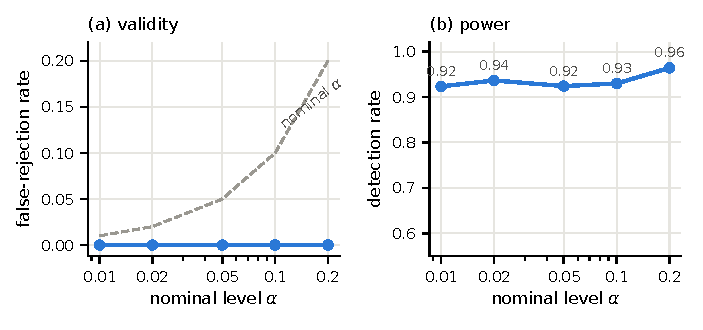
\includegraphics[width=\linewidth]{figures/Fig2}
\caption{Validity and power across the operating range ($100$
replications per level, Kelly routing). (a) Empirical false-rejection
of faithful candidates sits at zero under the nominal-$\alpha$
diagonal at every level --- the guarantee is an upper bound and holds
with the conservative margin the composite null demands. (b)
Detection of mutants is flat in $\alpha$, the empirical face of the
logarithmic budget bound of Proposition~\ref{prop:budget}}
\label{fig:alpha}
\end{figure} First, the guarantee
of Theorem~\ref{thm:validity} is an upper bound, not a calibration
claim: ECLAIR promises \emph{at most} $\alpha$, and the observed
margin is the structural price of a composite null --- tier B cannot
false-alarm by proof, and tiers A/C bet against upper-bounded null
rates because the true rates are unknowable. Second, the flatness of
the detection curve is Proposition~\ref{prop:budget} in action:
rejection budgets grow only logarithmically as $\alpha$ tightens.

\subsection{Tier ablation: what each probe class buys}
\label{sec:ablation}

Table~\ref{tab:ablation} repeats the testbed with restricted probe
pools; Figure~\ref{fig:ablation} visualizes the two headline columns.

\begin{figure}[t]
\centering
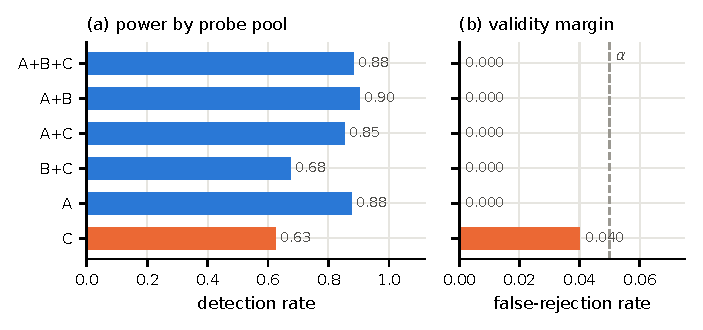
\includegraphics[width=\linewidth]{figures/Fig3}
\caption{Probe-tier ablation ($100$ replications per configuration,
Kelly, $\alpha=0.05$). (a) Detection by probe pool. (b) The validity
margin: every pool containing an unentangled tier (blue) records zero
false rejections; the pool-entangled cross-model tier alone (orange)
stays within $\alpha$ but consumes the entire conservative margin}
\label{fig:ablation}
\end{figure}

\begin{table}[t]
\caption{Probe-tier ablation ($100$ replications/configuration,
Kelly, $\alpha = 0.05$).}\label{tab:ablation}
\begin{tabular}{lccc}
\toprule
Tiers & False rej. & Detection & Kill cost\\
\midrule
A+B+C & $0.0000$ & $0.926$ & $21$\,ms\\
A+B   & $0.0000$ & $0.943$ & $21$\,ms\\
A+C   & $0.0000$ & $0.821$ & $17$\,ms\\
B+C   & $0.0000$ & $0.709$ & $36$\,ms\\
A     & $0.0000$ & $0.954$ & $21$\,ms\\
C     & $0.0401$ & $0.631$ & $71$\,ms\\
\bottomrule
\end{tabular}
\end{table}

Three findings. \emph{(i) Entanglement consumes the conservative
margin.} Every configuration containing an unentangled tier records
zero false rejections; tier C alone records $0.0401$ --- still within
$\alpha = 0.05$, but with the margin that conservative calibration
provides everywhere else fully spent. This is the empirical face of
the Remark after Proposition~\ref{prop:mr}: cross-model probes are
safe as a supplement, and their calibration must be conditioned on
pool composition before they can carry certification alone.
\emph{(ii) Hard certificates matter beyond their rate.} Removing tier
B (A+C vs.\ A+B+C) costs about ten points of detection although
tier-B alarms occur on only ${\sim}4\%$ of mutant probes.
\emph{(iii) A caveat on tier A's dominance.} Tier A alone detects
$95\%$ here, but mutation screening guarantees every mutant is
micro-instance-detectable --- precisely tier A's regime. Errors of
LLM origin need not be (conventions that diverge only at scale;
see below), which is why the tiered design is retained.

\subsection{External baselines at matched budget}\label{sec:baselines}

The routing policies of Table~\ref{tab:testbed} are internal
ablations; this section compares against the strategies a
practitioner would actually reach for, all given the \emph{same}
solver budget per pool and, where applicable, the same calibrated
null-rate bound $\bar p_0$. \emph{Single-shot} accepts the first
candidate unexamined. \emph{Self-consistency majority} solves all
candidates on eight shared instances and accepts the one agreeing
most often with the per-instance modal value --- the standard
LLM-ensemble heuristic; it has no rejection concept.
\emph{Fixed-sample} runs $n = 8$ cross-model probes per candidate and
rejects when the alarm count reaches the exact binomial critical
value at level $\alpha$ under $\bar p_0$ --- a textbook-valid test if
its assumptions hold. \emph{Peeking} applies that same binomial test
after every probe at nominal $\alpha$, stopping at the first crossing
--- the uncorrected sequential usage that testing loops drift into in
practice. \emph{Split conformal} rejects when the candidate's alarm
count is extreme against a $200$-run faithful calibration sample
($p_{\mathrm{conf}} \le \alpha$). Table~\ref{tab:baselines} reports
$100$ replications.

\begin{table}[t]
\caption{External baselines at matched budget ($100$ replications,
$\alpha = 0.05$). Only the e-process framework combines validity with
high power; the two fixed-sample-style tests break their nominal
level under family transfer and peeking respectively, and the
vote-based strategies cannot reject at all.}\label{tab:baselines}
\begin{tabular}{lccc}
\toprule
Method & False rej. & Detection & Pick acc.\\
\midrule
ECLAIR (Kelly, all tiers) & $\mathbf{0.0000}$ & $\mathbf{0.905}$ & $\mathbf{0.970}$\\
single-shot        & $0.0000$ & $0.000$ & $0.535$\\
self-consistency majority & $0.0000$ & $0.000$ & $0.879$\\
fixed-sample (tier C, $n{=}8$) & $0.0612$ & $0.578$ & $0.714$\\
peeking (tier C, uncorrected)  & $0.0748$ & $0.601$ & ---\\
split conformal (tier C)       & $0.0238$ & $0.480$ & ---\\
\bottomrule
\end{tabular}
\end{table}

Three comparisons carry the argument. \emph{Against vote-based
acceptance}: majority voting picks a faithful model $88\%$ of the
time but certifies unfaithful ones the remaining $12\%$ with no
warning, rejects nothing, and offers no level to quote; single-shot
is the coin flip its $0.535$ suggests. \emph{Against fixed-sample
testing}: the binomial test is nominally valid under its assumptions,
yet realizes $0.0612 > \alpha$ here --- the same cross-family
transfer and pool entanglement that the e-process absorbs
(Section~\ref{sec:ablation}: even tier-C-only stayed at $0.0401$)
push a hard accept/reject threshold over its level, because a
fixed-sample test has no supermartingale slack to spend. Its peeking
variant, the de-facto practice in iterative loops, inflates further
to $0.0748$ --- the canonical optional-stopping failure, here
measured rather than merely invoked. \emph{Against conformal}: with
an honest faithful-only calibration sample the conformal test keeps
its level ($0.0238$) but detects barely half of what ECLAIR does at
the same budget ($0.480$ vs.\ $0.905$), because a fixed probe count
cannot concentrate effort where evidence is accumulating. Matched
budget, same probes, same calibration information --- the difference
is purely the accounting.

\subsection{End-to-end study with real LLMs}\label{sec:llm}

Thirty candidates were generated from natural-language specifications
of the five families: two model families accessed through OpenRouter
(a free-tier routed model and \texttt{nvidia/nemotron-3-ultra-550b})
$\times$ three prompt styles (direct; restate-then-model; expert
persona) $\times$ per-style temperatures. Generated code is executed
in a sandboxed namespace; an intake gate requires each candidate to
build and solve two micro-instances. For scoring only, a proxy
faithfulness label compares each candidate against the enumeration
oracle on twelve micro-instances. All prompts, raw responses, and the
response cache are included in the supplementary material, and this
paragraph constitutes the documentation of LLM use in this study's
methods.

\emph{Generation.} $20/30$ candidates passed intake
(Table~\ref{tab:llm}). All ten failures were \emph{loud}: API
hallucinations importing conventions from other modelling ecosystems
--- \texttt{cp.Binary} and \texttt{cp.binary\_var} (PuLP/DOcplex
idioms), \texttt{cp.Var}, \texttt{cp.multiply},
\texttt{IntVar(domain=...)} (Choco-style),
\texttt{Model().NewBoolVar} (raw CP-SAT API), a bare
\texttt{import cp} --- each caught by the gate at negligible cost.
The failure mass is unevenly distributed: the large dedicated model
produced valid CPMpy for $14/15$ prompts, while the free-tier routed
model managed $6/15$, failing on entire families (generalized
assignment $0/3$) --- candidate diversity across model families is
what keeps such correlated failure from starving a pool.

\begin{table}[t]
\caption{End-to-end LLM study: intake outcomes per family and model
family ($3$ prompt styles each). Every intake failure is an API
hallucination caught by the gate; every intake survivor was
proxy-faithful.}\label{tab:llm}
\begin{tabular}{lccl}
\toprule
Family & routed free & nemotron-ultra & failure modes (intake)\\
\midrule
Knapsack+conflicts & $2/3$ & $3/3$ & \texttt{cp.Binary}\\
Set cover          & $1/3$ & $3/3$ & \texttt{cp.Binary}, \texttt{cp.multiply}\\
Graph colouring    & $2/3$ & $3/3$ & \texttt{IntVar(domain=...)}\\
Gen.\ assignment   & $0/3$ & $3/3$ & \texttt{cp.Var} ($\times 2$), \texttt{cp.binary\_var}\\
On-time selection  & $1/3$ & $2/3$ & \texttt{import cp}, \texttt{NewBoolVar}, runtime \texttt{None}\\
\midrule
Total              & $6/15$ & $14/15$ & \\
\bottomrule
\end{tabular}
\end{table}

\emph{Certification.} All $20$ intake survivors were proxy-faithful,
so the certified pools are all-null: the correct behaviour is to
reject nothing, and that is what happened --- $0/20$ false rejections
under every routing policy, the certified pick was faithful in all
five families, no abstentions, and no e-BH false discoveries. The
guarantee of Theorem~\ref{thm:validity} thus survives contact with
real generated models, complementing the mutation testbed in which
the same machinery demonstrably detects $87$--$94\%$ of actual
faults.

Two honest observations shape the outlook. On well-pinned
specifications, these two model families fail loudly (crashes) rather
than silently (wrong models) --- so the certification layer's
detection power is insurance whose premium, by
Proposition~\ref{prop:budget}, is logarithmically cheap. And
provoking the silent-error regime in LLM candidates requires
deliberately ambiguous, convention-laden specifications (the
colouring objective convention --- ``number of colours'' vs.\
``maximum colour index'' --- is the template), which is exactly where
ECLAIR's abstention-with-evidence output becomes the interesting
object of study; we return to this in Section~\ref{sec:limits}.

\subsection{Robustness: families, transfer direction, pool
composition}\label{sec:robustness}

Three sweeps probe whether the headline numbers are artifacts of a
particular experimental slice ($100$ replications each, Kelly,
$\alpha = 0.05$; Table~\ref{tab:robust}). \emph{Per family}: validity
is exact in every evaluation family separately; detection varies with
family difficulty ($0.99$ for set cover and $0.97$ for on-time
selection against $0.74$ for generalized assignment, whose
cost-matrix mutations produce the subtlest optimum shifts) --- power
is problem-dependent, the guarantee is not. \emph{Reversed
calibration split}: recalibrating on the three former evaluation
families and evaluating on knapsack$+$colouring yields false
rejection $0.0000$ with detection $0.804$ ($n = 309$ faithful) ---
cross-family transfer of the conservative bounds is bidirectional,
not an artifact of which families happened to calibrate.
\emph{Pool size and routing prior}: across $k \in \{4, 6, 10\}$ and
routing priors $q_{\mathrm{prior}} \in \{0.3, 0.5, 0.7\}$, false
rejection stays at $0.0000$ while detection moves only through the
router's aggressiveness (a pessimistic prior under-probes, $0.74$; a
suspicious one probes harder, $0.92$) --- the router's belief state
touches power alone, never the level, exactly as
Theorem~\ref{thm:validity} promises for any predictable routing.

\begin{table}[t]
\caption{Robustness sweeps ($100$ replications per row, Kelly,
$\alpha = 0.05$).}\label{tab:robust}
\begin{tabular}{llcc}
\toprule
Sweep & Configuration & False rej. & Detection\\
\midrule
family & set cover & $0.0000$ & $0.990$\\
family & generalized assignment & $0.0000$ & $0.743$\\
family & on-time selection & $0.0000$ & $0.971$\\
transfer & reversed calibration split & $0.0000$ & $0.804$\\
pool & $k = 4$ & $0.0000$ & $0.934$\\
pool & $k = 10$ & $0.0000$ & $0.893$\\
prior & $q_{\mathrm{prior}} = 0.3$ & $0.0000$ & $0.741$\\
prior & $q_{\mathrm{prior}} = 0.7$ & $0.0000$ & $0.920$\\
\bottomrule
\end{tabular}
\end{table}

\subsection{Probing the silent-error regime: ambiguous
specifications}\label{sec:ambiguity}

The main LLM study's lesson --- loud failures, faithful survivors ---
raises the question of whether \emph{silent} misreadings can be
elicited at all. We rephrased three specifications to plant boundary
ambiguities, fixed one canonical reading in the reference checker,
and regenerated candidate pools (both model families, three prompt
styles each): colouring with the objective convention sentence
\emph{removed} (``minimize the number of colors used''), knapsack
with ``the selected items together must be lighter than the
capacity'' (strict vs.\ non-strict), and on-time selection with
``every selected job is finished before its deadline'' (strict vs.\
non-strict completion).

The outcome is a negative result we report with its explanation:
$10/18$ generations passed intake, and \emph{all ten} implemented the
canonical reading --- no silent other-reading model appeared.
Certification behaved correctly throughout ($0/10$ false rejections,
canonical pick in $3/3$ families, no abstention). Two mechanisms
account for the miss. First, one planted ambiguity is
value-equivalent at the optimum: a model minimizing the \emph{count}
of distinct colours and one minimizing $1 + \max$ index return the
same optimal value on every instance, by precisely the renumbering
argument of Appendix~\ref{app:proofs} --- the readings differ only
off-optimum, where no value-level probe looks. Second, for the strict
/ non-strict boundary pairs, current models normalize aggressively to
the conventional reading ($\le$): the training distribution of
textbook formulations evidently dominates the literal text. The
constructive lesson for the elicitation agenda
(Section~\ref{sec:limits}) is that silent LLM errors are unlikely to
hide in boundary conventions; structural underspecification ---
omitted side constraints, ambiguous aggregation, units --- is the
more promising hunting ground, and value-equivalent ambiguities
require solution-level (not optimum-level) probes, which the
framework accommodates as additional tier-A checkers.

\subsection{Routing under heterogeneous probe costs}
\label{sec:heterogeneity}

The CP-SAT testbed's probes all cost single-digit milliseconds, which
compresses the routing question. To isolate it, a controlled
simulation reproduces the certification layer with the measured
alarm-rate structure but a $20{:}1$ probe-cost spread (expensive
near-exact oracles vs.\ cheap noisy checks --- the regime of
industrial instances, of costly solver calls, and of LLM-as-judge
probes priced per token). Over $500$ replications
(Figure~\ref{fig:routing}): Kelly routing detects $86\%$ of
unfaithful candidates at mean cost $12.2$ budget units per kill,
against $60\%$ at $16.6$ for round-robin and $77\%$ at $22.6$ for
cost-blind selection --- while false rejection stays at
$0.000$--$0.003$, below $\alpha$ for every policy. Routing gains
scale with probe-cost heterogeneity; validity is routing-invariant,
as Theorem~\ref{thm:validity} requires.

\begin{figure}[t]
\centering
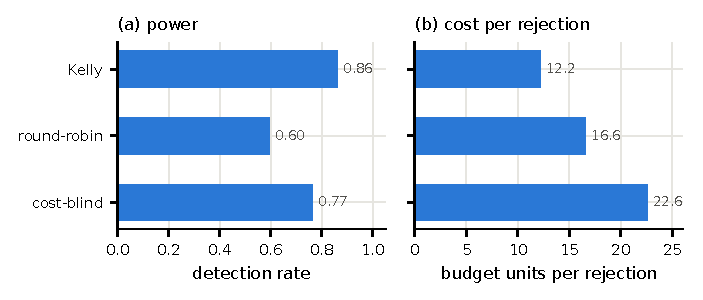
\includegraphics[width=\linewidth]{figures/Fig4}
\caption{Routing under a $20{:}1$ probe-cost spread ($500$
replications, $\alpha = 0.05$; measured alarm-rate structure,
controlled costs). Kelly routing dominates on both detection (a) and
budget per rejection (b); false-rejection stays below $\alpha$ under
every policy, as validity is routing-invariant}
\label{fig:routing}
\end{figure}

\section{Deployment guidance}\label{sec:deploy}

Because every quantity in the framework is operational, the knobs a
deploying team must set reduce to four, each with a concrete rule.

\paragraph{The level $\alpha$.} By Proposition~\ref{prop:budget} and
Figure~\ref{fig:alpha}, tightening $\alpha$ costs only logarithmic
budget and essentially no detection --- so $\alpha$ should be chosen
by the downstream stakes (what fraction of wrongly discarded faithful
models, and wrongly certified survivors under e-BH, the application
tolerates), not by compute anxiety. We used $0.05$ throughout; $0.01$
behaved identically.

\paragraph{The calibration corpus.} Validity consumes exactly one
number per noisy tier: an upper confidence bound $\bar p_0$ on the
null alarm rate. With zero observed false alarms in $n$ calibration
trials, the Clopper--Pearson bound scales as
$\bar p_0 \approx 3.7/n$ ($n{=}100$: $0.036$; $n{=}240$: $0.015$;
$n{=}1000$: $0.0037$), and a smaller $\bar p_0$ buys a larger alarm
multiplier $p_1/\bar p_0$ --- calibration effort converts directly
into per-alarm evidence. Known-faithful models for the corpus are the
cheap part: hand-written reference models on any families adjacent to
the deployment domain suffice, and our results show the bounds
transfer across families when used conservatively.

\paragraph{The budget.} The testbed's operating point --- ${\sim}80$
mean-cost probes per pool of six --- put the marginal probe well past
the detection plateau. The budget-to-rejection bound gives the
back-of-envelope sizing rule: expect
${\sim}\log(1/\alpha)/\Delta$ probes per unfaithful candidate, with
$\Delta$ the per-probe expected log-evidence (${\approx}1.5$ for our
calibrated tier A under $\hat p_1 \approx 0.6$), so single-digit
probes per rejection --- consistent with the measured $20$\,ms kill
costs against $5$\,ms probes.

\paragraph{What to log.} The evidence ledger --- every probe, its
tier, instance seed, outcome, and e-factor --- is the audit object:
it makes each rejection reproducible (replay the counterexample),
each certification quantifiable (survived evidence at level
$\alpha$), and each abstention actionable (which readings died on
which probes). Teams wrapping an existing agentic modelling loop
\cite{szeider2025cpagent, szeider2025mcp} need to intercept only two
things: candidate model source and solver calls.

\section{Threats to validity}\label{sec:threats}

\emph{Internal.} The statistical guarantee rests on
Assumption~\ref{ass:null}; the ablation localizes exactly where its
tier-A/C half is fragile (pool-entangled probes carrying sole
weight) and the baselines show the failure is not hypothetical ---
the same miscalibration that leaves the e-process at $0.040$ pushes a
fixed-sample threshold to $0.061$. Tier-B validity is by proof, but
only for relations proved against the \emph{specification}; a
relation read off a formulation can be invalid
(Section~\ref{sec:library}).

\emph{Construct.} Mutation screening makes every testbed fault
micro-detectable, biasing tier importance toward A
(Section~\ref{sec:ablation}); proxy faithfulness labels in the LLM
studies are themselves enumeration-based and share this bias. The
ambiguity study is the counterweight, since other-reading models
differ precisely where enumeration on canonical micro-instances says
they do.

\emph{External.} Two model families, five problem families, one
modelling language: claims about ``LLM modellers'' beyond these are
extrapolation. The error taxonomy (Table~\ref{tab:llm}) will age as
models improve; the framework's premise --- that whatever errors
remain be caught with a guarantee --- does not depend on the
taxonomy's contents.

\section{Limitations and outlook}\label{sec:limits}

\emph{Calibration scope.} Validity rests on
Assumption~\ref{ass:null}; our evidence that conservative calibration
transfers across problem families is empirical (zero false rejections
under family transfer), not a theorem, and tier-C calibration should
be conditioned on pool composition before cross-model evidence
carries substantial weight --- the ablation shows the margin, though
never the bound, giving way. \emph{Screened mutants.} The testbed's
faults are guaranteed micro-detectable by construction; LLM-native
silent errors need not be, and eliciting them requires deliberately
ambiguous specifications --- the planned abstention study, which also
connects certification to conversational elicitation. \emph{Checker
provenance.} Our enumeration checkers are hand-written and
independent; a fully LLM-generated pipeline must calibrate
checker error as tier-A noise, which the framework accommodates but
this study does not exercise. \emph{Breadth.} Five families suffice
to exercise every mechanism; scaling the probe library toward
CSPLib/NL4Opt breadth, and stating the MR validity results for global
constraints (\texttt{alldifferent}, \texttt{cumulative}) in the
generality they deserve, are the natural next steps.
\emph{Beyond one modelling language.} Nothing in the framework is
CPMpy-specific: candidates are opaque functions from instances to
optima, so MiniZinc, MILP, or SMT candidates certify identically ---
indeed a heterogeneous pool (the same specification modelled in CP
\emph{and} MILP) strengthens tier C precisely because formalism
diversity decorrelates errors. What each new language requires is an
exact solve at micro/mid scale and, for tier B, relations proved
against the specification; the three relation classes of
Section~\ref{sec:library} are formalism-independent.
\emph{Eliciting silent errors.} The ambiguity study
(Section~\ref{sec:ambiguity}) shows boundary conventions are
normalized away by current models and value-equivalent readings are
invisible to optimum-level probes; the elicitation agenda should
target structural underspecification, and the probe pool should grow
solution-level checkers where readings coincide in value but not in
argmax.

\section{Conclusion}\label{sec:conclusion}

ECLAIR turns the verification of LLM-generated constraint models from
a heuristic detection exercise into sequential hypothesis testing
with explicit guarantees: anytime-valid false-rejection control under
optional stopping and adaptive, budget-aware probe routing; FDR
control across a generate--test--repair tournament; and an auditable
evidence ledger for every decision, including abstention. On real
CP-SAT probes the guarantee held exactly at every operating level
while nine of ten injected faults were caught within sub-second
budgets, and the framework certified real LLM-generated models
without error. The broader claim is methodological: solver-in-the-loop
verification of generative models is, at bottom, a sequential
inference problem, and the e-process toolkit fits it exactly.

\backmatter

\section*{Statements and Declarations}

\textbf{Funding.} %% TODO(authors): confirm.
The authors did not receive support from any organization for the
submitted work.

\textbf{Competing interests.} %% TODO(authors): confirm.
The authors have no competing interests to declare that are relevant
to the content of this article.

\textbf{Data availability.} All code, calibration data, experimental
results, and cached LLM generations are available in the
supplementary material.
%% TODO(authors): public repository URL / archived DOI.

\textbf{Use of large language models.} LLMs are the object of study;
their use in the experiments (models, prompting, decoding parameters,
caching) is documented in Section~\ref{sec:llm}.
%% TODO(authors): decide and add the venue-appropriate statement on
%% AI-assisted manuscript preparation per Springer policy.

\begin{appendices}

\section{Validity proofs for the probe library}\label{app:proofs}

Throughout, $\mathcal{X}(I)$ denotes the specification's feasible set
on instance $I$, $f_I$ its objective, and
$v^\ast(I) = \mathrm{opt}_{x \in \mathcal{X}(I)} f_I(x)$. Because
tier-B probes solve the \emph{candidate} exactly on both sides, and a
faithful candidate satisfies $v_m \equiv v^\ast$, it suffices to
prove each relation for $v^\ast$. Three lemmas cover all but one
relation.

\begin{lemma}[Relaxation]\label{lem:relax}
If $\mathcal{X}(I) \subseteq \mathcal{X}(I')$ and $f_{I'} = f_I$,
then $v^\ast(I') \ge v^\ast(I)$ for maximization and
$v^\ast(I') \le v^\ast(I)$ for minimization.
\end{lemma}
\begin{proof}
The optimum over a superset is no worse: any $x$ optimal for $I$ is
feasible for $I'$ with the same objective value.
\end{proof}

\begin{lemma}[Objective dominance]\label{lem:dom}
If $\mathcal{X}(I') = \mathcal{X}(I)$ and
$f_{I'}(x) \ge f_I(x)$ for all $x \in \mathcal{X}(I)$, then
$v^\ast(I') \ge v^\ast(I)$, for maximization and minimization alike.
\end{lemma}
\begin{proof}
For maximization, dominate the maximizer of $I$; for minimization,
$\min_x f_{I'}(x) \ge \min_x f_I(x)$ since every point's value rose.
\end{proof}

\begin{lemma}[Symmetry]\label{lem:sym}
If $\pi$ is a bijection of the decision index set and $I'$ is $I$
with all indexed data consistently relabeled by $\pi$, then
$x \mapsto x \circ \pi^{-1}$ is a bijection
$\mathcal{X}(I) \to \mathcal{X}(I')$ preserving objective values;
hence $v^\ast(I') = v^\ast(I)$.
\end{lemma}
\begin{proof}
Every constraint and objective term of the specification refers to
indices only through the relabeled data, so feasibility and value are
preserved in both directions.
\end{proof}

\paragraph{Knapsack with conflicts (max).}
Capacity increase relaxes the single budget constraint
(Lemma~\ref{lem:relax}: $\uparrow$). Deleting a conflict pair removes
a constraint (Lemma~\ref{lem:relax}: $\uparrow$). Item permutation,
with the conflict list relabeled by the same permutation, is
Lemma~\ref{lem:sym}.

\paragraph{Set cover (min).}
Deleting an element removes one covering constraint
(Lemma~\ref{lem:relax}: $\downarrow$). Raising one set's cost is
Lemma~\ref{lem:dom} on a minimization ($\uparrow$). Permuting the set
collection (costs and coverage lists together) is Lemma~\ref{lem:sym}.

\paragraph{Graph colouring (min).}
The specification minimizes the number of colours; the implemented
objective, $1 + \max_i c_i$ over proper colourings with colours in
$\{0, \dots, n-1\}$, agrees with it at the optimum because any proper
colouring with $k$ distinct colours can be renumbered onto
$\{0, \dots, k-1\}$ without violating properness. Edge deletion
removes a disequality constraint (Lemma~\ref{lem:relax}:
$\downarrow$); edge addition adds one, shrinking the feasible set
(Lemma~\ref{lem:relax} applied with the roles of $I, I'$ exchanged:
$\uparrow$); vertex relabeling is Lemma~\ref{lem:sym}.

\paragraph{Generalized assignment (min).}
Raising one machine's capacity relaxes its load constraint
(Lemma~\ref{lem:relax}: $\downarrow$). Raising one cost entry is
Lemma~\ref{lem:dom} ($\uparrow$). Task permutation (sizes and cost
rows together) is Lemma~\ref{lem:sym}.

\paragraph{On-time job selection (max).}
This is the delicate family. The specification selects
$S \subseteq \{1, \dots, n\}$ maximizing $\sum_{j \in S} w_j$ subject
to \emph{schedulability}: some single-machine order completes every
job of $S$ by its deadline. The classical characterization states
that $S$ is schedulable iff processing $S$ in nondecreasing-deadline
(EDD) order is feasible, iff
\begin{equation}\label{eq:edd}
\textstyle\sum_{i \in S:\, d_i \le d_j} p_i \;\le\; d_j
\qquad \text{for every } j \in S .
\end{equation}
\emph{Weight increase} is Lemma~\ref{lem:dom} ($\uparrow$).
\emph{Processing-time decrease}: in any fixed order every completion
time weakly decreases, so every schedulable $S$ remains schedulable;
the feasible set (in the schedulability sense) grows, and
Lemma~\ref{lem:relax} gives $\uparrow$. \emph{Deadline increase}
$d_k \mapsto d_k + \delta$: note that the index sets in
\eqref{eq:edd} change with the deadline order, so monotonicity of the
inequality system is not syntactic. Argue at the schedulability
level instead: fix a schedule witnessing feasibility of $S$ under the
old deadlines; completion times are unchanged and deadlines are
pointwise no smaller, so the same schedule witnesses feasibility
under the new deadlines. Hence every schedulable set remains
schedulable, and Lemma~\ref{lem:relax} gives $\uparrow$; the
candidate, if faithful, satisfies \eqref{eq:edd} on both sides
because \eqref{eq:edd} is equivalent to schedulability instance by
instance. Job permutation (processing times, deadlines, and weights
together) is Lemma~\ref{lem:sym}. \qed

\section{Natural-language specifications and prompts}
\label{app:prompts}

For reproducibility, the exact specification texts and the prompt
template of the end-to-end study (Section~\ref{sec:llm}). Candidates
were requested as a single Python function
\texttt{build\_model(params)} returning a CPMpy model with the
objective set, under three style hints --- \emph{direct} (``Write the
model directly.'', temperature $0.3$), \emph{stepwise} (``First
restate the decision variables, constraints and objective in one
short paragraph each, then write the code.'', $0.7$), and
\emph{expert} (``You are an expert constraint-programming modeller
known for scrupulously faithful formalizations. Write the model.'',
$0.5$).

\paragraph{Template.}
\begin{quote}\small\ttfamily
Translate the following optimization problem into a CPMpy model.\\[2pt]
\{SPECIFICATION\}\\[2pt]
\{STYLE HINT\}\\[2pt]
Requirements: provide a single Python function build\_model(params)
that returns a cpmpy.Model with the objective set (use
model.maximize(...) or model.minimize(...)); use only the cpmpy
library (imported as cp) and the Python standard library; the
function must work for ANY params dict matching the schema; reply
with ONLY a Python code block.
\end{quote}

\paragraph{Specification texts (abridged schema lines).}
Knapsack with conflicts: \emph{``You must select a subset of $n$
items. Item $i$ has weight $w[i]$ and value $v[i]$. The total weight
of selected items must not exceed the capacity cap. Some pairs of
items conflict: for each pair $(i,j)$ in the list conflicts, items
$i$ and $j$ must not both be selected. Maximize the total value of
the selected items.''} Set cover: \emph{``There are nelem elements,
numbered $0..\mathrm{nelem}-1$, and a collection of sets. Set $s$
covers the elements listed in sets$[s]$ and costs cost$[s]$. Choose a
sub-collection of sets so that every element is covered by at least
one chosen set. Minimize the total cost of the chosen sets.''} Graph
colouring: \emph{``Color the $n$ vertices of an undirected graph,
using color indices from $0$ to $n-1$, so that the two endpoints of
every edge receive different colors. Minimize the number of colors
used. IMPORTANT convention: the objective value must equal $1$ plus
the maximum color index used.''} Generalized assignment:
\emph{``Assign each of $T$ tasks to exactly one of $M$ machines. Task
$t$ has size $p[t]$; machine $m$ has capacity cap$[m]$: the total
size of tasks assigned to machine $m$ must not exceed cap$[m]$.
Assigning task $t$ to machine $m$ costs cost$[t][m]$. Minimize the
total assignment cost.''} On-time job selection: \emph{``A single
machine processes jobs one at a time. Job $j$ has processing time
$p[j]$, deadline $d[j]$ and weight $wt[j]$. Select a subset of jobs
that can ALL be completed by their deadlines when the selected jobs
are processed in non-decreasing deadline order (equivalently: a
selected set is feasible if and only if, for every selected job $j$,
the sum of processing times of selected jobs $i$ with
$d[i] \le d[j]$ is at most $d[j]$). Maximize the total weight of the
selected jobs.''}

The colouring convention sentence is deliberate: without it,
``minimize the number of colors'' admits the objective
$|\{c_i\}|$ as a faithful reading, and the two readings differ only
off-optimum --- the template for the planned ambiguous-specification
study (Section~\ref{sec:limits}).

\section{The mutation operator catalogue}\label{app:mutations}

Each operator is a deterministic function of instance parameters,
drawn once per candidate and applied identically to every instance
the candidate ever sees (a wrong \emph{model}, not a wrong instance).
Descriptors are sampled uniformly over the applicable
(operator, target) pairs of Table~\ref{tab:families}; positional
indices are drawn once and taken modulo the current instance's
dimension, which is what makes them instance-generic.

\begin{description}
\item[scalar shift] a named scalar bound $b \mapsto \max(1, b+\delta)$,
  $\delta \in \{\pm 1, \pm 2, \pm 3\}$ (misread constant).
\item[vector entry] one positionally selected entry of a named
  numeric vector shifted by $\delta$ as above (misread datum).
\item[vector rotation] a named vector rotated by one position ---
  the data-wiring misalignment in which item $i$ receives item
  $(i{+}1)$'s datum; the mutation class that only the permutation MR
  and value-level oracles can see.
\item[row drop] one positionally selected structural row (conflict
  pair, edge, coverage list) deleted (missed constraint).
\item[family half-drop] the second half of a structural family
  deleted (systematically missed constraint class).
\item[matrix entry] one positionally selected entry of a cost matrix
  shifted by $\delta$.
\item[operator flip] one constraint family's comparison direction
  inverted at the builder level ($\le \leftrightarrow \ge$; for
  colouring, disequality to equality) --- the class that breaks
  monotone MRs and is otherwise invisible to agreement checks when
  the flipped model is infeasible-prone.
\end{description}

\emph{Screening.} A drawn mutant is kept only if its exact optimum
differs from the specification's brute-forced optimum on at least one
of six random micro-instances (up to $40$ redraws); this discards
semantically equivalent mutants, the standard practice in mutation
testing, and guarantees ground-truth labels for every experiment in
Section~\ref{sec:experiments}.

\section{Extended numerical tables}\label{app:tables}

For re-derivation without running code, the full operating-range
table behind Figure~\ref{fig:alpha} ($100$ replications per level,
Kelly routing; kill cost is mean measured solver time to reject a
mutant):

\begin{table}[h]
\caption{Full $\alpha$-sweep.}\label{tab:alphafull}
\begin{tabular}{lccccc}
\toprule
$\alpha$ & false rej. & $n$ faithful & detection & $n$ mutants & kill cost\\
\midrule
$0.01$ & $0.0000$ & $300$ & $0.923$ & $300$ & $30.5$\,ms\\
$0.02$ & $0.0000$ & $285$ & $0.937$ & $315$ & $30.0$\,ms\\
$0.05$ & $0.0000$ & $297$ & $0.924$ & $303$ & $22.8$\,ms\\
$0.10$ & $0.0000$ & $301$ & $0.930$ & $299$ & $19.4$\,ms\\
$0.20$ & $0.0000$ & $293$ & $0.964$ & $307$ & $20.7$\,ms\\
\bottomrule
\end{tabular}

The kill-cost column is Proposition~\ref{prop:budget} measured:
tightening the guarantee from $\alpha = 0.20$ to $\alpha = 0.01$ ---
a $20\times$ stronger error bound --- raises the mean solver cost of
a rejection from ${\sim}21$\,ms to ${\sim}30$\,ms, a factor of
${\sim}1.5$, in line with the predicted
$\log(1/0.01)/\log(1/0.20) \approx 2.9$ ratio of log-thresholds
attenuated by hard-certificate rejections whose cost is
$\alpha$-independent.
\end{table}

Calibrated betting multipliers implied by Table~\ref{tab:calib}
(equation~\eqref{eq:bet}): tier A alarm $\times 30.9$, pass
$\times 0.535$; tier C alarm $\times 3.00$, pass $\times 0.607$;
tier B pass $\times 1$, alarm $= \infty$. Rejection threshold at
$\alpha = 0.05$: wealth $20$, i.e.\ $\log$-threshold $3.00$.

\section{Complete generation record}\label{app:genrecord}

Every LLM generation across both studies (main: Section~\ref{sec:llm};
ambig: Section~\ref{sec:ambiguity}), in request order. ``free'' is
the free-tier routed model; ``nemotron'' is
\texttt{nvidia/nemotron-3-ultra-550b}; error classes abbreviate the
exception type raised at the intake gate (AttrErr:
\texttt{AttributeError}, ModErr: \texttt{ModuleNotFoundError},
TypeErr: \texttt{TypeError}, SynErr: \texttt{SyntaxError}); the raw
responses ship in the supplementary cache.

\begin{table}[h]
\caption{All 48 generations.}\label{tab:genrecord}
\footnotesize
\begin{tabular}{llllll}
\toprule
Study & Family & Model & Style & Intake & Outcome / error\\
\midrule
main & knapsack\_conflicts & free & direct & fail & \texttt{AttrErr}\\
main & knapsack\_conflicts & free & stepwise & ok & faithful\\
main & knapsack\_conflicts & free & expert & ok & faithful\\
main & knapsack\_conflicts & nemotron & direct & ok & faithful\\
main & knapsack\_conflicts & nemotron & stepwise & ok & faithful\\
main & knapsack\_conflicts & nemotron & expert & ok & faithful\\
main & set\_cover & free & direct & fail & \texttt{AttrErr}\\
main & set\_cover & free & stepwise & ok & faithful\\
main & set\_cover & free & expert & fail & \texttt{AttrErr}\\
main & set\_cover & nemotron & direct & ok & faithful\\
main & set\_cover & nemotron & stepwise & ok & faithful\\
main & set\_cover & nemotron & expert & ok & faithful\\
main & coloring & free & direct & ok & faithful\\
main & coloring & free & stepwise & ok & faithful\\
main & coloring & free & expert & fail & \texttt{TypeErr}\\
main & coloring & nemotron & direct & ok & faithful\\
main & coloring & nemotron & stepwise & ok & faithful\\
main & coloring & nemotron & expert & ok & faithful\\
main & gen\_assignment & free & direct & fail & \texttt{AttrErr}\\
main & gen\_assignment & free & stepwise & fail & \texttt{AttrErr}\\
main & gen\_assignment & free & expert & fail & \texttt{AttrErr}\\
main & gen\_assignment & nemotron & direct & ok & faithful\\
main & gen\_assignment & nemotron & stepwise & ok & faithful\\
main & gen\_assignment & nemotron & expert & ok & faithful\\
main & ontime\_selection & free & direct & fail & \texttt{ModErr}\\
main & ontime\_selection & free & stepwise & fail & \texttt{AttrErr}\\
main & ontime\_selection & free & expert & ok & faithful\\
main & ontime\_selection & nemotron & direct & ok & faithful\\
main & ontime\_selection & nemotron & stepwise & ok & faithful\\
main & ontime\_selection & nemotron & expert & fail & \texttt{AttrErr}\\
\midrule
ambig & coloring & free & direct & fail & \texttt{SynErr}\\
ambig & coloring & free & stepwise & fail & \texttt{ModErr}\\
ambig & coloring & free & expert & fail & \texttt{AttrErr}\\
ambig & coloring & nemotron & direct & ok & canonical\\
ambig & coloring & nemotron & stepwise & fail & \texttt{AttrErr}\\
ambig & coloring & nemotron & expert & ok & canonical\\
ambig & knapsack\_conflicts & free & direct & fail & no code block\\
ambig & knapsack\_conflicts & free & stepwise & fail & \texttt{AttrErr}\\
ambig & knapsack\_conflicts & free & expert & fail & no code block\\
ambig & knapsack\_conflicts & nemotron & direct & ok & canonical\\
ambig & knapsack\_conflicts & nemotron & stepwise & ok & canonical\\
ambig & knapsack\_conflicts & nemotron & expert & ok & canonical\\
ambig & ontime\_selection & free & direct & ok & canonical\\
ambig & ontime\_selection & free & stepwise & ok & canonical\\
ambig & ontime\_selection & free & expert & fail & \texttt{AttrErr}\\
ambig & ontime\_selection & nemotron & direct & ok & canonical\\
ambig & ontime\_selection & nemotron & stepwise & ok & canonical\\
ambig & ontime\_selection & nemotron & expert & ok & canonical\\
\bottomrule
\end{tabular}
\end{table}

\end{appendices}

\bibliography{references}

\end{document}
